\documentclass[11pt]{article} 

% packages with special commands
\usepackage{amssymb, amsmath}
\usepackage{epsfig}
\usepackage{array}
\usepackage{ifthen}
\usepackage{color}
%\usepackage{fancyhdr}
\usepackage{graphicx}
\usepackage{indentfirst}
\usepackage{caption}
%\usepackage{mathtools}
\definecolor{grey}{rgb}{0.5,0.5,0.5}

\begin{document}
\newcommand{\tr}{\text{tr}}
\newcommand{\E}{\textbf{E}}
\newcommand{\diag}{\text{diag}}
\newcommand{\argmax}{\text{argmax}}
\newcommand{\argmin}{\text{argmin}}
\newcommand{\Cov}{\text{Cov}}
\newcommand{\Var}{\text{Var}}
\newcommand{\Vol}{\text{Vol}}
\newcommand{\HH}{\boldsymbol{H}}
%\pagestyle{fancy}

\begin{center}
\begin{tabular}{ccc}
$v_0 = 2, \omega_0 = 0.5$ & $v_0 = 2.01, \omega_0 = 0.5$ & $v_0 = 2.1, \omega_0 = 0.5$\\
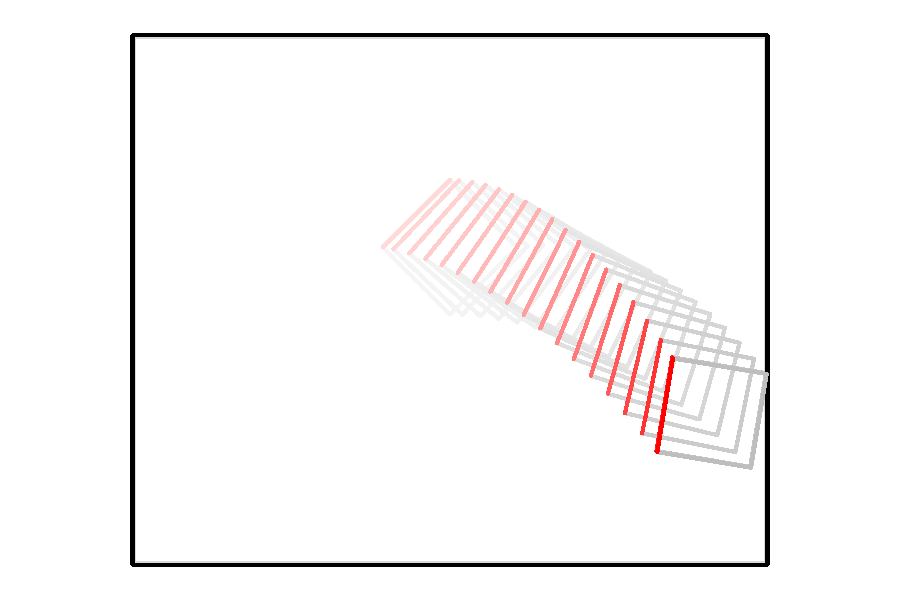
\includegraphics[scale = 0.26]{simA_01.pdf} & 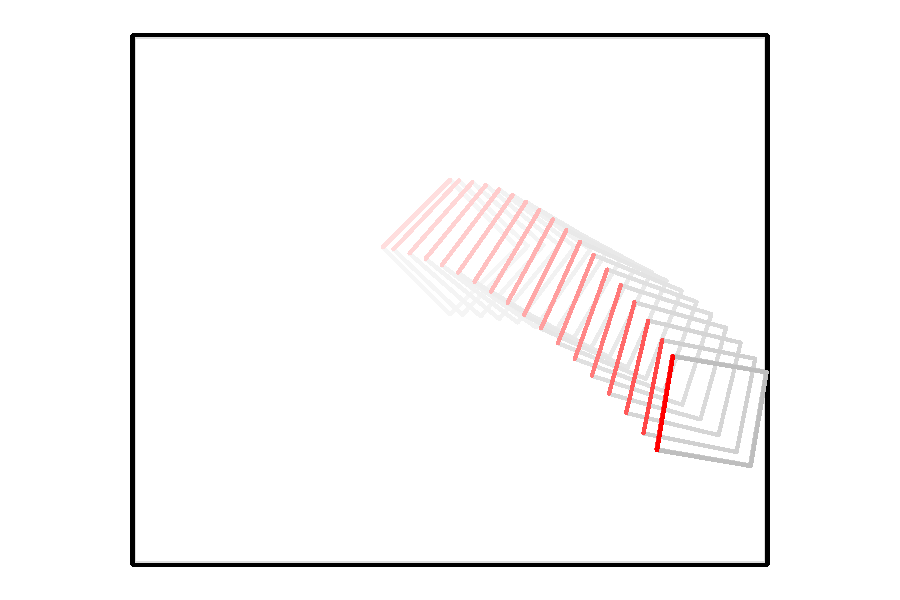
\includegraphics[scale = 0.26]{simB_01.pdf} & 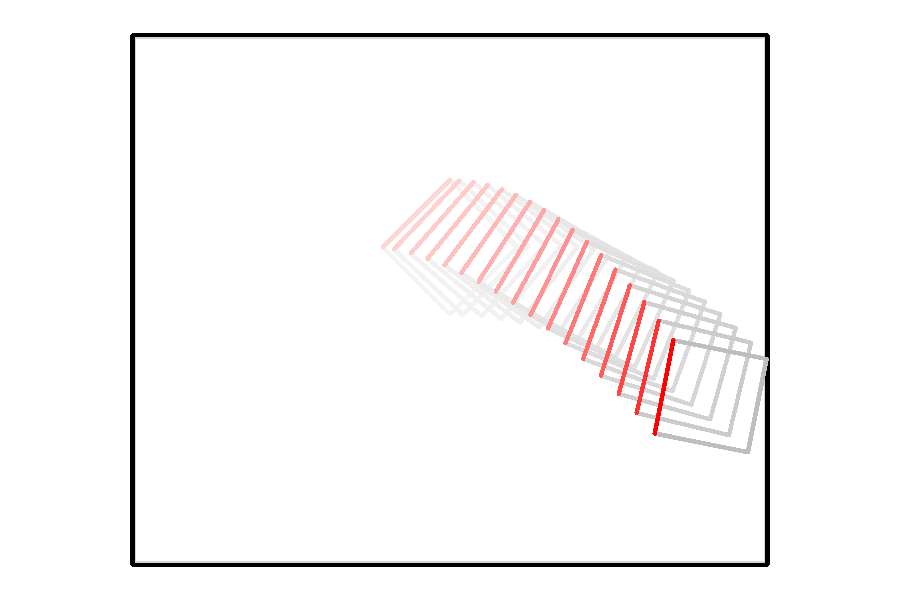
\includegraphics[scale = 0.26]{simC_01.pdf} \\
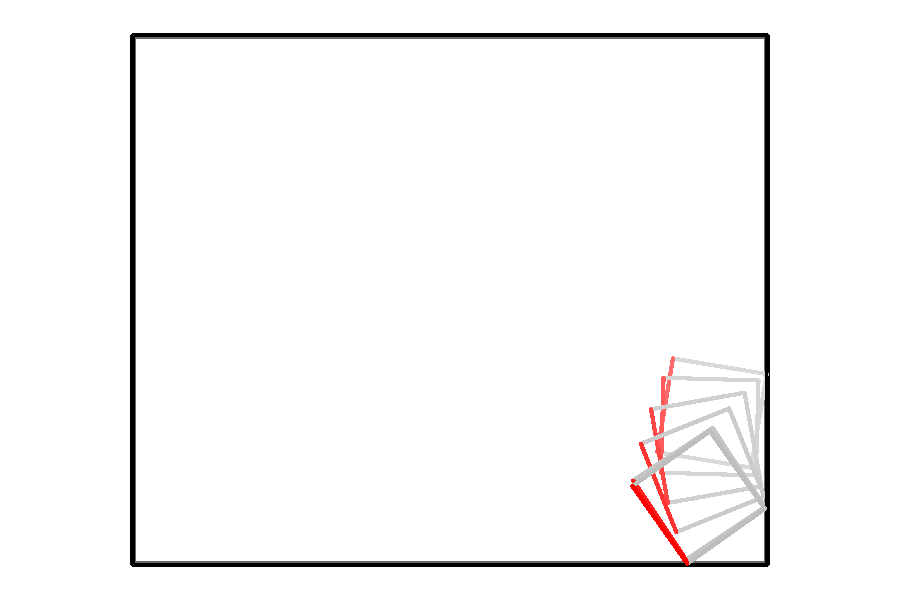
\includegraphics[scale = 0.26]{simA_02.pdf} & 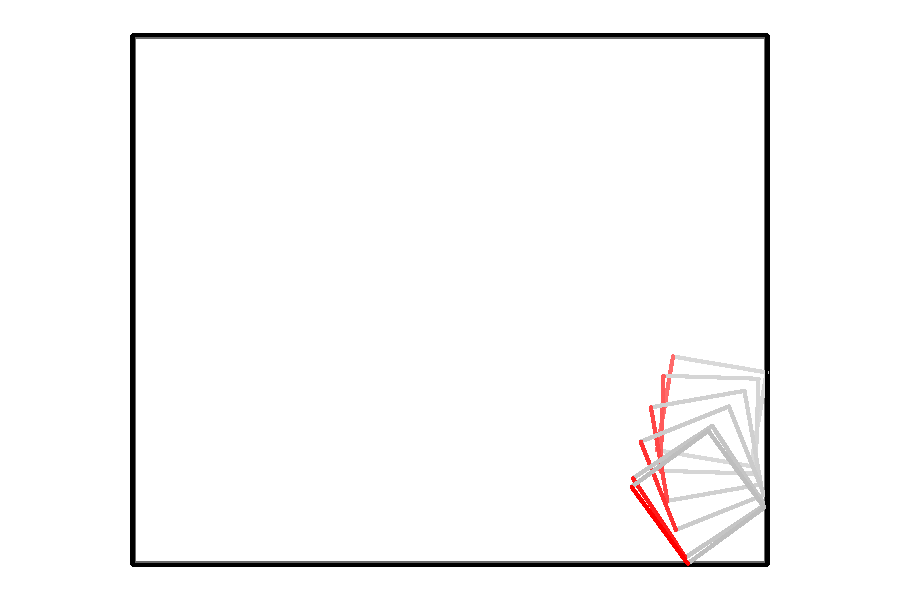
\includegraphics[scale = 0.26]{simB_02.pdf} & 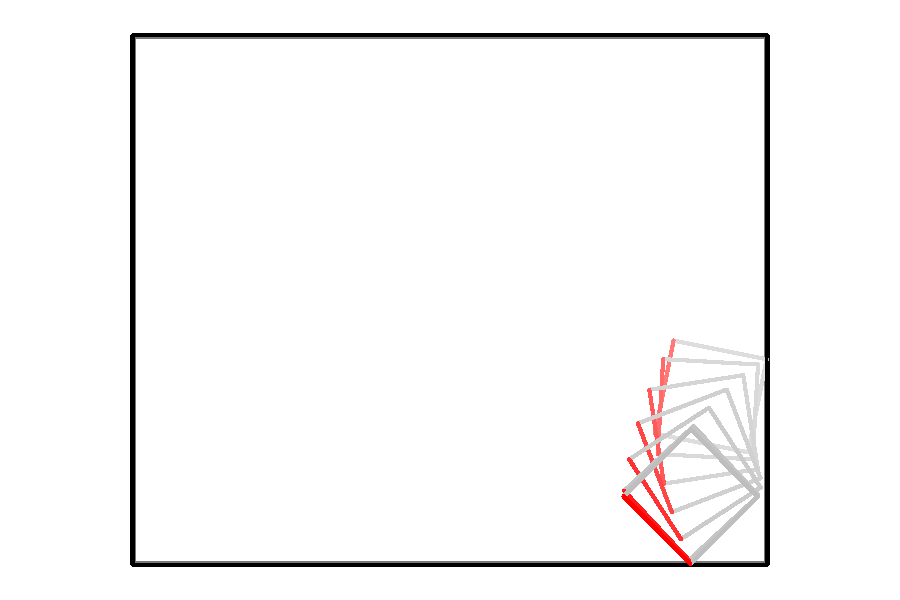
\includegraphics[scale = 0.26]{simC_02.pdf} \\
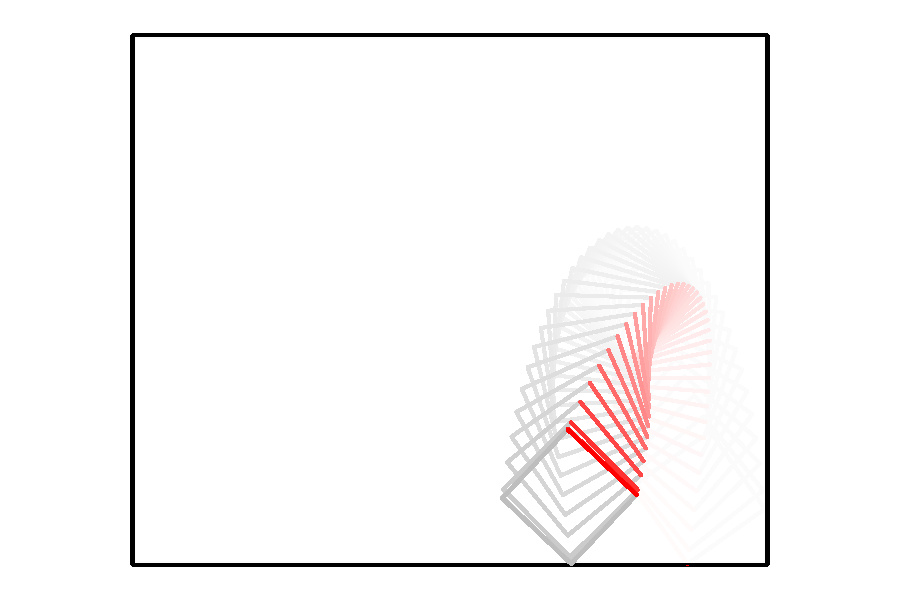
\includegraphics[scale = 0.26]{simA_03.pdf} & 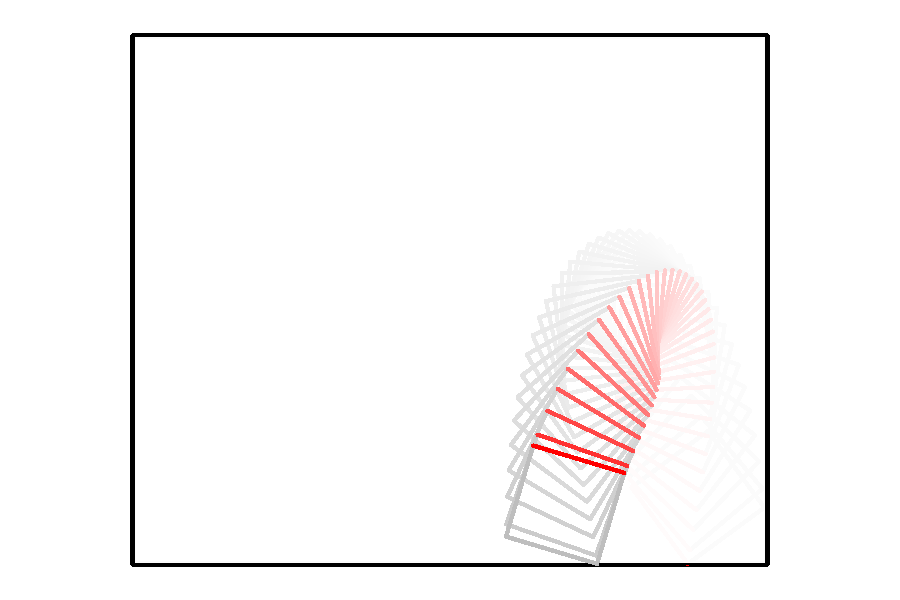
\includegraphics[scale = 0.26]{simB_03.pdf} & 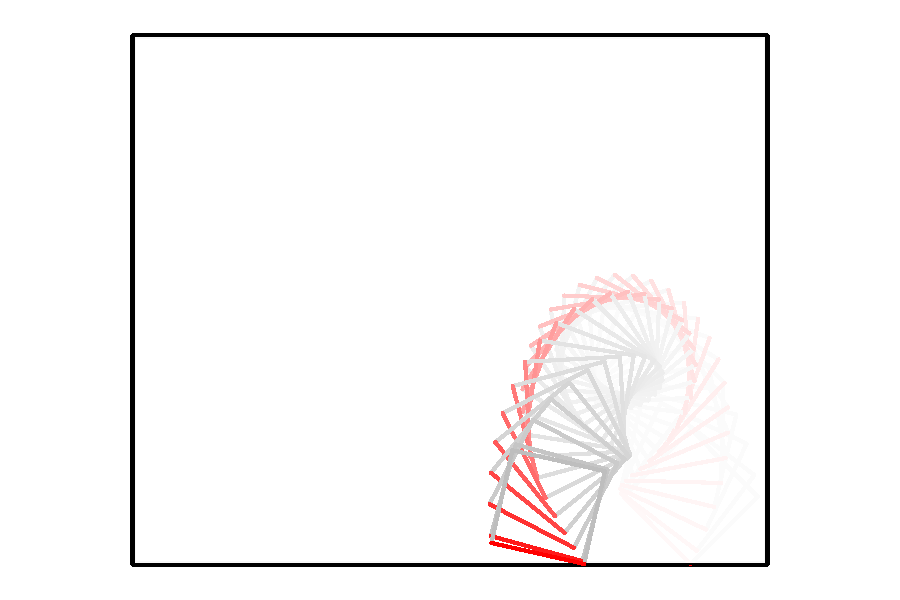
\includegraphics[scale = 0.26]{simC_03.pdf} \\
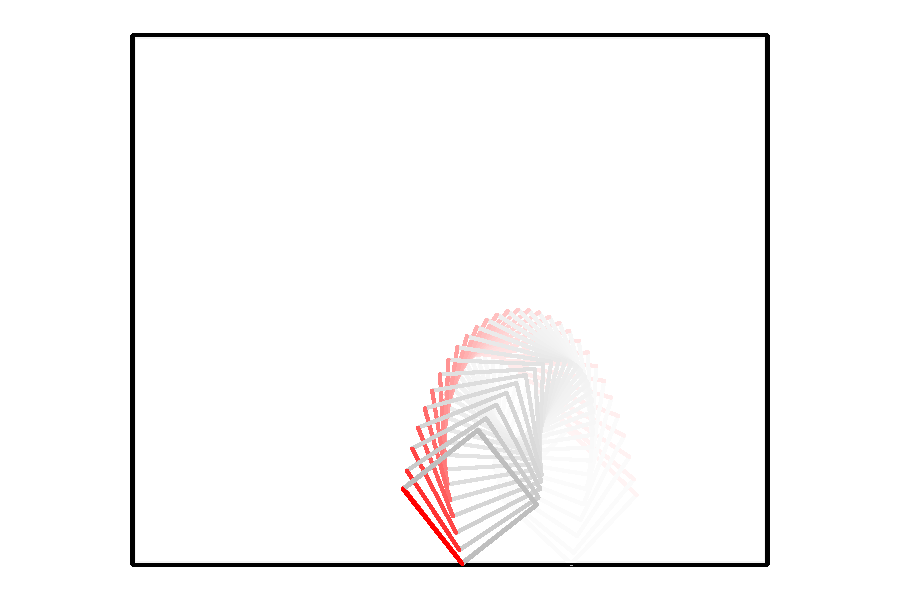
\includegraphics[scale = 0.26]{simA_04.pdf} & 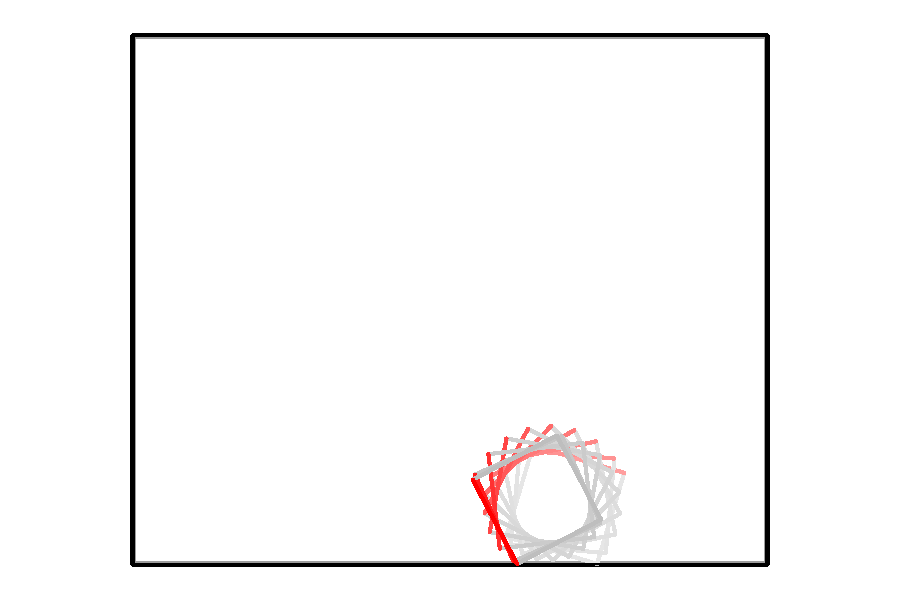
\includegraphics[scale = 0.26]{simB_04.pdf} & 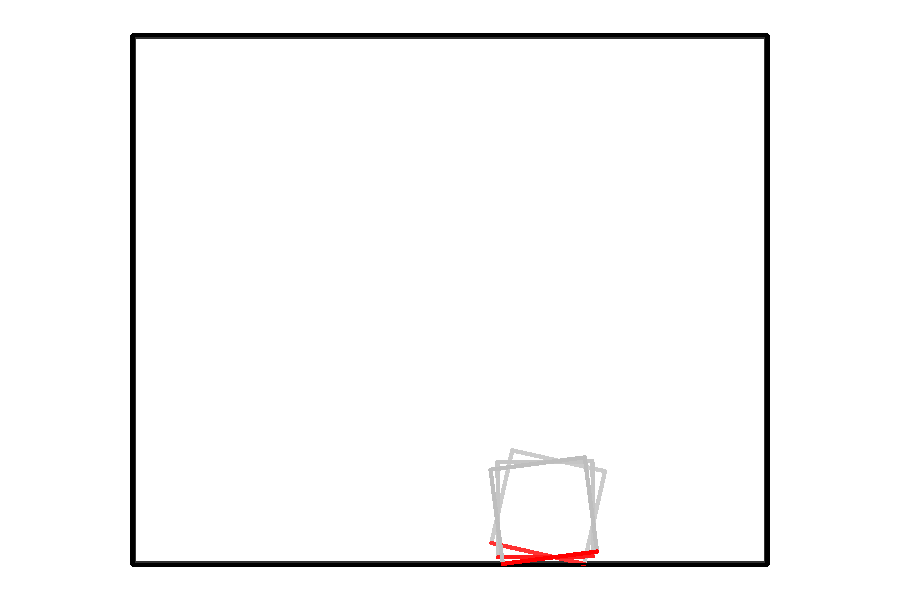
\includegraphics[scale = 0.26]{simC_04.pdf} \\
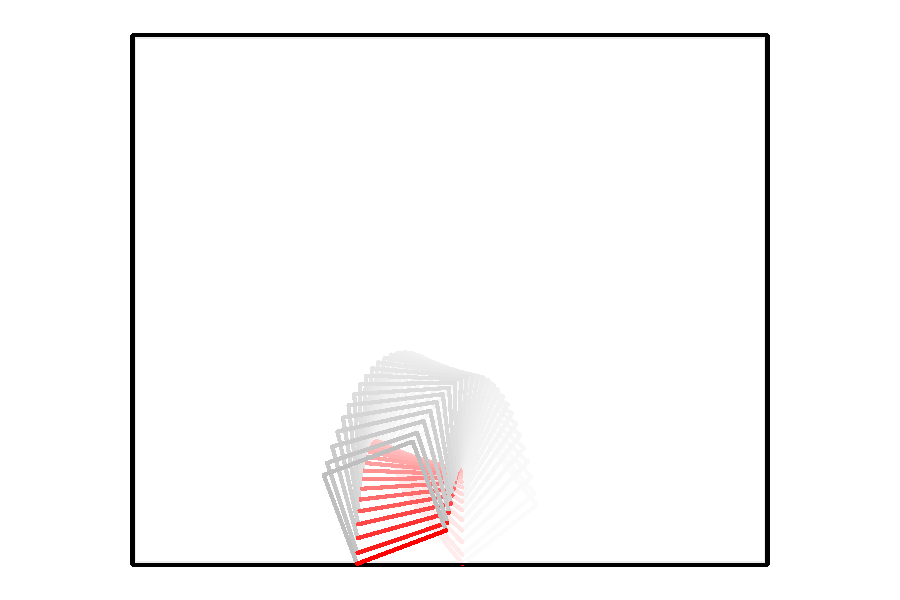
\includegraphics[scale = 0.26]{simA_05.pdf} & 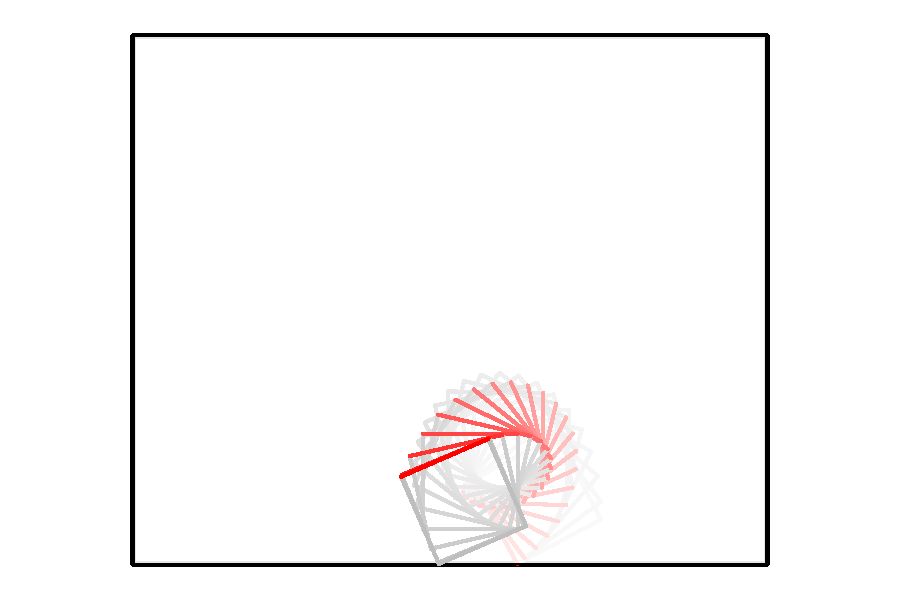
\includegraphics[scale = 0.26]{simB_05.pdf} & 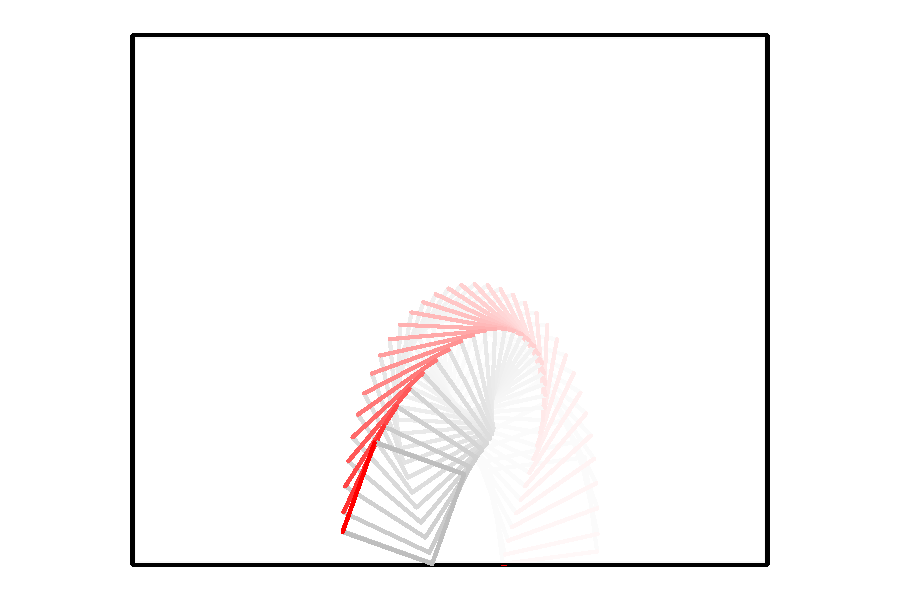
\includegraphics[scale = 0.26]{simC_05.pdf} \\
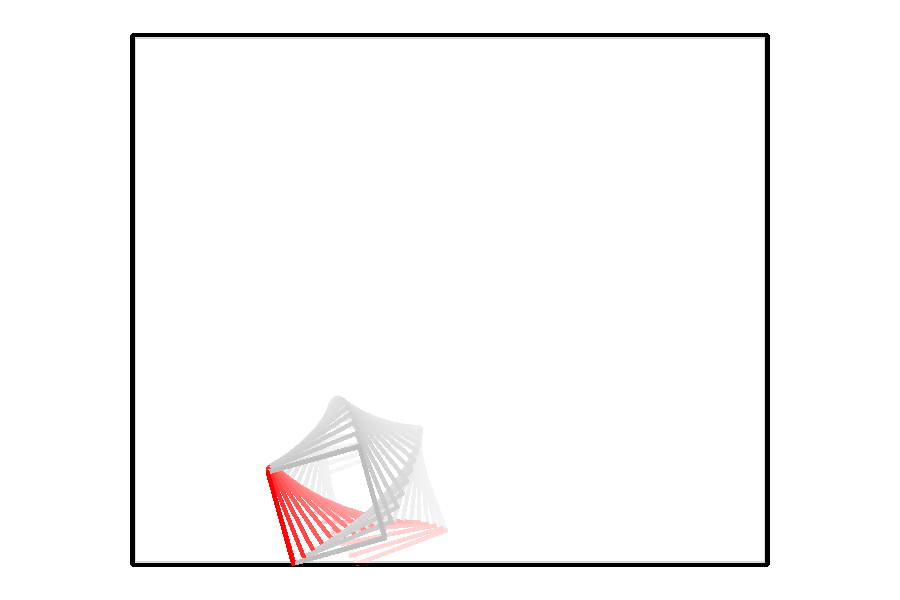
\includegraphics[scale = 0.26]{simA_06.pdf} & 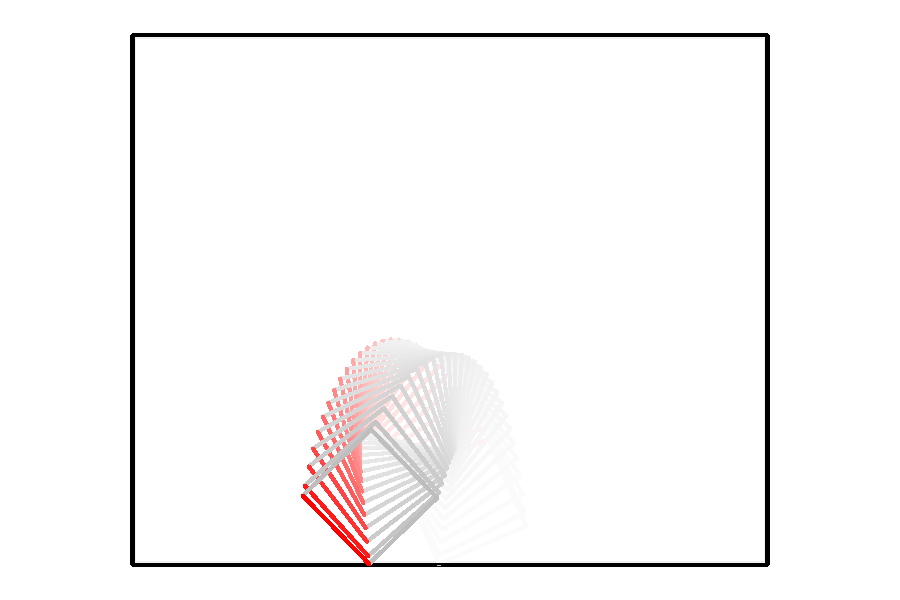
\includegraphics[scale = 0.26]{simB_06.pdf} & 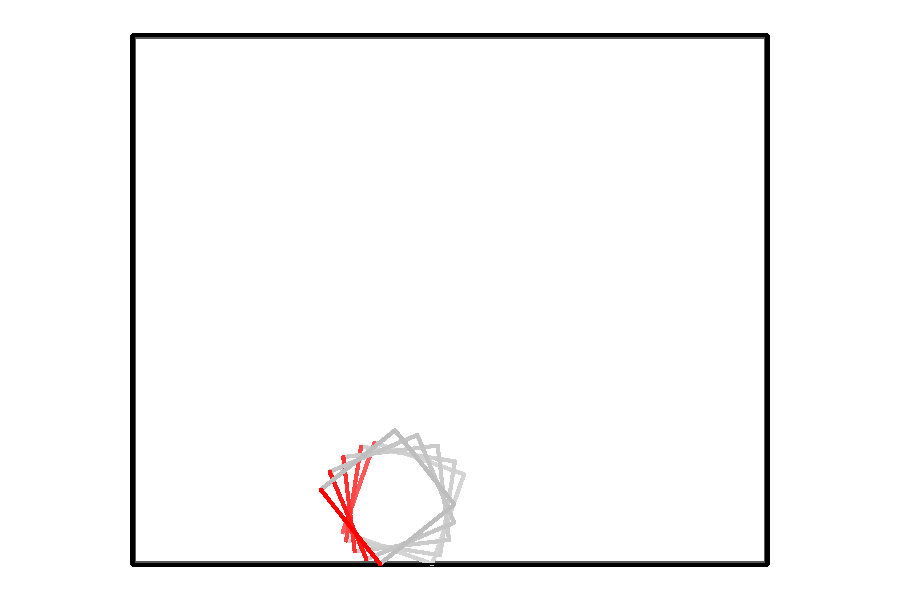
\includegraphics[scale = 0.26]{simC_06.pdf} \\
\end{tabular}
\end{center}

\end{document}
